\chapter{Opis projektnog zadatka}
		
		\textbf{\textit{dio 1. revizije}}\\
		
		Cilj ovog projekta je razviti programsku podršku za stvaranje web aplikacije "Eventio", koja će korisnicima omogućiti stvaranje, oglašavanje i sudjelovanje na različitim događanjima. Ova inovativna web aplikacija će korisnicima omogućiti lakši pristup društevnim događanjima koja odgovaraju njihovim interesima te olakšati organizaciju i promociju istih.
		
		Postoje mnoge društvene platforme koje već imaju razvijene mreže korisnika i nude vlastite implementacije sličnih rješenja za događanja. Međutim, ono što "Eventio" čini drugačijim jest njegov pristup. Dok druga rješenja ovise o korisnicima koji stvaraju različite grupe i objavljuju događanja na koje se korisnici prijavljuju ili postaju članovi tih grupa (primjer toga je Facebook), "Eventio" nudi alternativni pristup. Korisnici će moći vidjeti sve dostupne događaje i filtrirati ih prema vlastitim preferencama, kao što su vrsta događaja, lokacija, datum i druge karakteristike. Na taj način, korisnici će imati veće šanse saznati za događanja koja najbolje odgovaraju njihovim interesima, čime se rješava glavni problem: pronalaženje događanja koja odgovaraju njihovim željama i potrebama.
		
		Ova aplikacija je namijenjena svima - bez obzira na dob, spol ili interes. Svatko tko želi sudjelovati na događanjima bilo kojeg opsega i pronaći svoju zajednicu s istim interesima može pronaći korist u "Eventio". Osim što korisnicima pruža bolji pristup događanjima, aplikacija također nudi organizatorima priliku da promoviraju svoje događaje i privuku veći broj sudionika.
		
		Unatoč prednostima, postoji nekoliko problema koji će se morati rješavati kako bi se projekt uspješno realizirao i u konačnici našao među krajnjim korisnicima. Aplikacija ovisi o velikom broju korisnika i organizatora kako bi postala funkcionalna i privukla interes. Potrebno je privući dovoljan broj organizatora s raznovrsnim događanjima kako bi se zadovoljili interesi široke publike. Također, potrebno je privući i potaknuti korisnike da koriste aplikaciju i aktivno sudjeluju na događanjima. Konkurencija s postojećim sličnim rješenjima kao što su Facebook, Meetup i Eventbrite ima prednost zbog svojih već razvijenih korisničkih baza koje mogu koristiti za testiranje i lansiranje ovakvog proizvoda.
		
		U ovom kontekstu, "Eventio" se postavlja kao platforma koja će pružiti jednostavan i učinkovit način povezivanja organizatora i posjetitelja događanja te olakšati promociju i sudjelovanje u raznovrsnim događanjima. Kroz inovativan pristup i kontinuirane nadogradnje, "Eventio" ima potencijal promijeniti način na koji korisnici pronalaze i sudjeluju na događanjima u svom okruženju.
		Primarni cilj ovog zadatka je razviti Minimalan vitalni proizvod (Minimum viable product, MVP), rješenje koje će na najjednostavniji i pristupačan način rješavati problem pronalaženja i sudjelovanja na događanjima prema osobnim preferencama. MVP će osigurati osnovne funkcionalnosti aplikacije kako bi se zadovoljile osnovne potrebe korisnika i omogućila provedba testiranja i daljnjeg razvoja.
		
		U sljedećem dijelu opisa projekta bit će detaljno razrađena problematika zadatka. Također, bit će opisani korisnički zahtjevi i predložena moguća rješenja za svaku komponentu aplikacije. Sve ovo ima za cilj definirati temelje i smjernice za daljnji razvoj "Eventio" aplikacije.
		
		Sljedeći dio opisa projekta detaljnije će razmotriti problematiku projektnog zadatka, identificirati glavne aktere i dionike te opisati korisničke zahtjeve i funkcionalnosti aplikacije "Eventio".
		
		Glavni akteri uključuju:
		\begin{packed_item}
			\item \textit{Administrator: Osoba s najvišim ovlastima u sustavu, odgovorna za upravljanje korisnicima, događajima, i financijskim aspektima}
			\item \textit{Korisnik (Organizator): Osoba koja može stvarati i oglašavati svoje događaje, upravljati svojim profilom, i platiti mjesečnu članarinu za objavu plaćenih događaja}
			\item \textit{Korisnik (Posjetitelj): Osoba koja može pretraživati i iskazivati zainteresiranost za događaje, ostavljati recenzije i upravljati svojim profilom.}
			\item \textit{Banka i PayPal: Pruzatelji usluga placanja koji omogucuju korisnicima placanje mjesečne članarine i ulaznica za događaje.}
			\item \textit{Baza podataka: Skladište podataka o korisnicima, događajima, recenzijama, i financijskim transakcijama}
		\end{packed_item}
		
		Sada ćemo detaljnije razmotriti korisničke zahtjeve i funkcionalnosti aplikacije "Eventio".
		
		Prilikom pokretanja aplikacije, korisniku će se prikazati jedna od dvije mogućnosti. 
		
		\begin{packed_item}
			\item \textit{Prozor sa pozdravom: Korisnik je već stvorio profil i ranije se prijavio u sustav}
			\item \textit{Prozor sa formom za prijavu te gumbom koji vodi na kreiranje novog računa: Ovisno o tome posjeduje li korisnik račun će ili ispuniti prijavu u sustav ili pak kliknuti na gumb za stvaranje računa. }
		\end{packed_item}
		 Kako bi korisnik mogao uspješno kreirati račun potrebni su sljedeći podaci:
		\begin{packed_item}
			\item \textit{Korisničko ime}
			\item \textit{Lozinka}
			\item \textit{E-mail adresa}
		\end{packed_item}
		Korisnik tijekom registracije isto tako može birati koju ulogu želi imati unutar aplikacije. Uloge su posjetitelj i organizator.
		Ako je korisnik odabrao ulogu organizatora, tada još dodatno uz navedene podatke treba upisati i sljedeće:
		\begin{packed_item}
			\item \textit{Naziv organizacije}
			\item \textit{Adresa}
			\item \textit{Link/Url svoje stranice}
		\end{packed_item}
		
		Nakon kreiranja samog računa kao jedna uloga, neće biti omogućeno mijenjanje  te uloge. 
		Za prijavu će biti potrebno unijeti korisničko ime i lozinku postojećeg računa. Za odjavu će korisnici imati gumb odjavi koji je potrebno pritisnuti kako bi se korisnik odjavio sa računa te se nakon toga vraća na početni zaslon sa formom za prijavu.
		
		Nakon uspješne prijave/registracije kao organizator događaja, korisnik može krenuti sa oglašavanjem. Prilikom unosa novog događaja, organizator mora unijeti podatke kao što su: 
		\begin{packed_item}
			\item \textit{Naziv događaja}
			\item \textit{Vrsta događaja}
			\item \textit{Lokacija događaja}
			\item \textit{Opis lokacije}
			\item \textit{Vrijeme početka}
			\item \textit{Trajanje}
			\item \textit{Cijena ulaznice}
			\item \textit{Opis događaja}
		\end{packed_item}
		
		Gore navedeni podaci su obavezni, te uz obavezne podatke organizator može dodati još slike ili video snimke u galeriju samog događaja. Kada završi sa kreiranjem događaja, njega je moguće vidjeti na profilu organizatora zajedno sa svim njegovim podacima te događajima koji su se zbili unatrag dvije godine ili drugim događajima koji su stvoreni i tek dolaze.
		
		Neki organizatori će organizirati događaje s besplatnim ulazom, no neki će vjerojatno htjeti naplatiti ulaz na događaj. Za mogućnost objavljivanja budućih događaja za koje se plaća ulaz organizator mora biti pretplatnik mjesečne članarine na web aplikaciji. Prilikom objave prvog takvog događaja organizator je obvezan platiti članarinu. 
		
		Članarina se može platiti na dva načina:
		\begin{packed_item}
			\item \textit{PayPal}
			\item \textit{Bankovna kartica}
		\end{packed_item}
		
		Članarina će se obnavljati na mjesečnoj bazi sve dokle organizator sadrži neki događaj za koji je potrebno plaćanje ulaza. Također, prilikom objave novog događaja od strane organizatora za koji se naplaćuje ulaz, a organizator je u tom trenutku pretplatnik, slobodan je objaviti događaj normalnim procesom bez dodatnih obaveza.
		
		Nakon uspješne prijave/registracije kao posjetitelj, korisnik može krenuti tražiti događaje koji mu odgovaraju te iskazivati svoju zainteresiranost za sami dolazak na te događaje. Zainteresiranost se dijeli u tri skupine: 
		\begin{packed_item}
			\item \textit{Sigurno dolazim}
			\item \textit{Možda dolazim}
			\item \textit{Ne dolazim}
		\end{packed_item}
		
		Kada korisnik stisne na bilo koju grupu, na samom događaju će biti vidljiva zainteresiranost. Ako je odabrana grupa „Sigurno dolazim“ ili „Možda dolazim“, tada se na profilu posjetitelja pojavi taj događaj. 
		
		Posjetitelj isto tako može ostaviti recenziju na događaju koja će biti dodana u listu svih recenzija pod tim događajem. Kako bi ju uspješno dodao u listu recenzija, svaka recenzija mora sadržavati kratki opis recenzije te opcionalno može sadržavati ocjenu od 1 do 10. 
		
		Posjetitelji unutar aplikacije mogu filtrirati sve događaje. Mogu ih filtrirati po nazivu ili vrsti događaja, njihovom vremenu početka, po lokaciji na kojoj se događaj odvija te po samom trajanju događaja. Na taj način posjetitelj može naći one događaje koji mu najviše odgovaraju i koji su mu najpogodniji. Kako bi se najvećim fanovima olakšala potražnja događaja njihovih najdražih organizatora, svaki posjetitelj moći će pretraživati isto tako i po korisničkom imenu organizatora. Kao što je navedeno, na profilu organizatora navedeni su svi prethodni događaji te svi događaji u budućnosti koji se također mogu filtrirati.
		
		Svaki korisnik će isto tako imati mogućnosti osvježavanja i uređivanja vlastitog profila. Posjetitelji će moći izmijeniti svoje podatke te uvijek mogu promijeniti zainteresiranost za neki event. Osim toga, posjetitelji mogu odabrati postavke da im aplikacija automatski šalje obavijesti o najnovijim događanjima prema zadanim kriterijima: vrsta događanja i područje. Organizatori uz promjene vlastitih podataka mogu isto tako promijeniti podatke događaja koji će se tek dogoditi, a svi oni već prošli događaji neće se moći mijenjati od strane organizatora. 
		
		Kako bi posjetiteljima dodatno olakšali korištenje aplikacije, događaji na kojima će zainteresiranost biti „Sigurno dolazim“ ili „Možda dolazim“ poslati će e-mail poruku na posjetiteljev račun 24 sata prije početka događaja. Isto tako, kada dođe do neke promjene na događaju, a koje nisu došle sa strane posjetitelja, ponovno stiže notifikacija u obliku e-mail poruke o samoj promjeni.
		
		Uz dvije uloge korisnika, organizator i posjetitelj, unutar sustava postoji i uloga administratora. Administrator se kao i ostali korisnici može prijaviti te odjaviti iz sustava te unutar sustava on je korisnik s najvišim ovlastima. 
		
		Neće imati mogućnosti iskazati zainteresiranost za neki event te neće moći stvarati događaje kao što to organizator može, no ima druge ovlasti. On može pristupiti bazi podataka te može pregledati profil bilo kojeg drugog korisnika. Ukoliko smatra potrebnim, on može mijenjati podatke o događajima te može brisati recenzije ukoliko ih smatra nevaljanim. Isto tako može brisati same događaje, ali i korisnike ako se ne pridržavaju pravila unutar aplikacije. Zajedno sa time, on je taj koji određuje kolika će biti cijena mjesečne članarine koju plaćaju organizatori koji posjeduju neki događaj za koji se plaća upad.
		
		Za ovakav tip proizvoda može se stalnim nadogradnjama i poboljšanjima privući još i šira publika. Ubrzo bi se na sami prototip aplikacije mogli dodati i chatovi unutar svakog događaja kako bi ljudi mogli komunicirati i prije samog događaja te na taj način zapravo započeli sami događaj i prije njegovog stvarnog početka. Uz ovaj dodatak mogli bi se na vrh svakog pretraživanja dodati i oni događaji za koje smatramo da su najpogodniji posjetitelju ovisno o njegovim prošlim izborima događaja. 
		
		
		\eject
		
		\section{Primjeri u \LaTeX u}
		
		\textit{Ovo potpoglavlje izbrisati.}\\

		U nastavku se nalaze različiti primjeri kako koristiti osnovne funkcionalnosti \LaTeX a koje su potrebne za izradu dokumentacije. Za dodatnu pomoć obratiti se asistentu na projektu ili potražiti upute na sljedećim web sjedištima:
		\begin{itemize}
			\item Upute za izradu diplomskog rada u \LaTeX u - \url{https://www.fer.unizg.hr/_download/repository/LaTeX-upute.pdf}
			\item \LaTeX\ projekt - \url{https://www.latex-project.org/help/}
			\item StackExchange za Tex - \url{https://tex.stackexchange.com/}\\
		
		\end{itemize} 	


		
		\noindent \underbar{podcrtani tekst}, \textbf{podebljani tekst}, 	\textit{nagnuti tekst}\\
		\noindent \normalsize primjer \large primjer \Large primjer \LARGE {primjer} \huge {primjer} \Huge primjer \normalsize
				
		\begin{packed_item}
			
			\item  primjer
			\item  primjer
			\item  primjer
			\item[] \begin{packed_enum}
				\item primjer
				\item[] \begin{packed_enum}
					\item[1.a] primjer
					\item[b] primjer
				\end{packed_enum}
				\item primjer
			\end{packed_enum}
			
		\end{packed_item}
		
		\noindent primjer url-a: \url{https://www.fer.unizg.hr/predmet/proinz/projekt}
		
		\noindent posebni znakovi: \# \$ \% \& \{ \} \_ 
		$|$ $<$ $>$ 
		\^{} 
		\~{} 
		$\backslash$ 
		
		
		\begin{longtblr}[
			label=none,
			entry=none
			]{
				width = \textwidth,
				colspec={|X[8,l]|X[8, l]|X[16, l]|}, 
				rowhead = 1,
			} %definicija širine tablice, širine stupaca, poravnanje i broja redaka naslova tablice
			\hline \SetCell[c=3]{c}{\textbf{naslov unutar tablice}}	 \\ \hline[3pt]
			\SetCell{LightGreen}IDKorisnik & INT	&  	Lorem ipsum dolor sit amet, consectetur adipiscing elit, sed do eiusmod  	\\ \hline
			korisnickoIme	& VARCHAR &   	\\ \hline 
			email & VARCHAR &   \\ \hline 
			ime & VARCHAR	&  		\\ \hline 
			\SetCell{LightBlue} primjer	& VARCHAR &   	\\ \hline 
		\end{longtblr}
		

		\begin{longtblr}[
				caption = {Naslov s referencom izvan tablice},
				entry = {Short Caption},
			]{
				width = \textwidth, 
				colspec = {|X[8,l]|X[8,l]|X[16,l]|}, 
				rowhead = 1,
			}
			\hline
			\SetCell{LightGreen}IDKorisnik & INT	&  	Lorem ipsum dolor sit amet, consectetur adipiscing elit, sed do eiusmod  	\\ \hline
			korisnickoIme	& VARCHAR &   	\\ \hline 
			email & VARCHAR &   \\ \hline 
			ime & VARCHAR	&  		\\ \hline 
			\SetCell{LightBlue} primjer	& VARCHAR &   	\\ \hline 
		\end{longtblr}
	


		
		
		%unos slike
		\begin{figure}[H]
			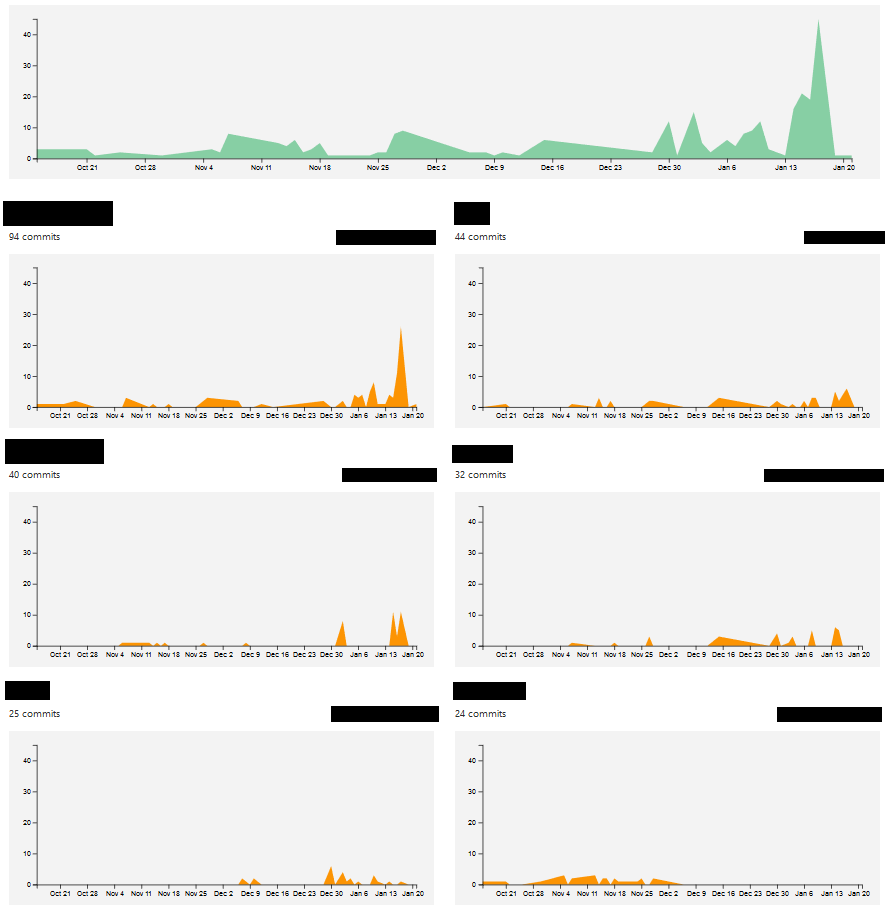
\includegraphics[scale=0.4]{slike/aktivnost.PNG} %veličina slike u odnosu na originalnu datoteku i pozicija slike
			\centering
			\caption{Primjer slike s potpisom}
			\label{fig:promjene}
		\end{figure}
		
		\begin{figure}[H]
			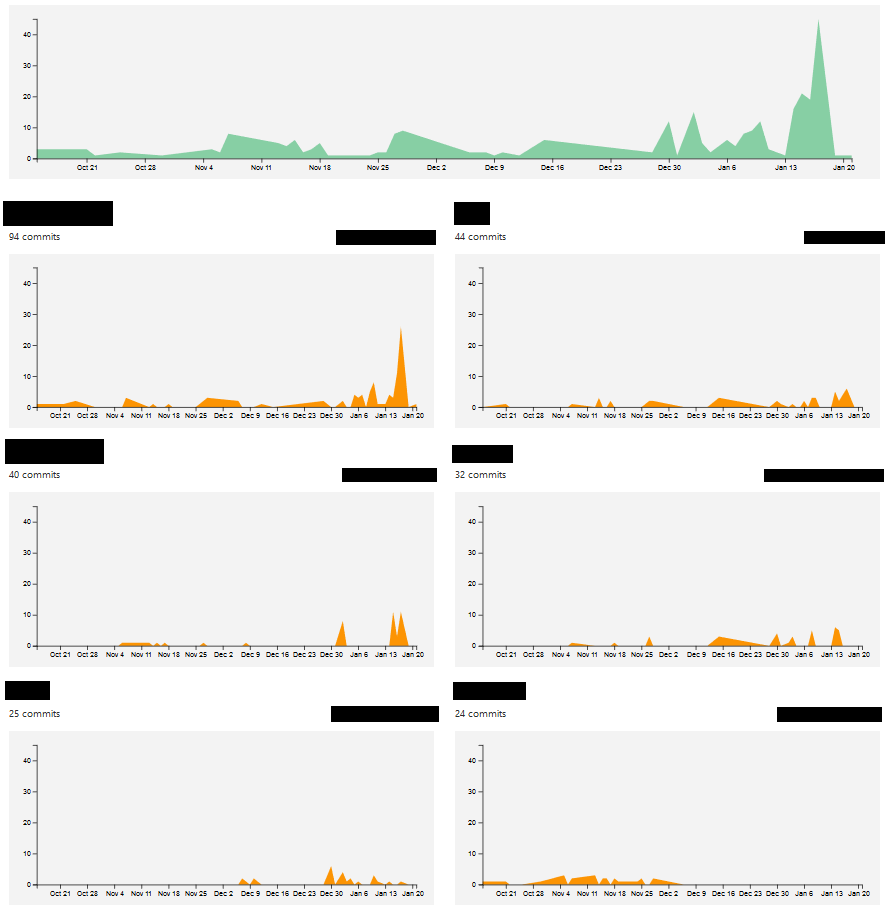
\includegraphics[width=\textwidth]{slike/aktivnost.PNG} %veličina u odnosu na širinu linije
			\caption{Primjer slike s potpisom 2}
			\label{fig:promjene2} %label mora biti drugaciji za svaku sliku
		\end{figure}
		
		Referenciranje slike \ref{fig:promjene2} u tekstu.
		
		\eject
		
	